\documentclass[10pt,a4paper,fleqn]{article}

%% my packages
\usepackage{a4wide}
\usepackage[round,longnamesfirst]{natbib}
\usepackage{hyperref}
%
\usepackage{amsmath}
\usepackage{amsfonts}
\usepackage[utf8]{inputenc}
%
\newcommand{\strong}[1]{{\normalfont\fontseries{b}\selectfont #1}}
\newcommand{\class}[1]{\mbox{\textsf{#1}}}
\newcommand{\func}[1]{\mbox{\texttt{#1()}}}
\newcommand{\code}[1]{\mbox{\texttt{#1}}}
\newcommand{\pkg}[1]{\strong{#1}}
\newcommand{\samp}[1]{`\mbox{\texttt{#1}}'}
\newcommand{\proglang}[1]{\textsf{#1}}
\newcommand{\set}[1]{\mathcal{#1}}

\usepackage{Sweave}
%% \VignetteIndexEntry{Introduction to TSP}



\begin{document}


\title{Introduction to \pkg{TSP} -- Infrastructure for the Traveling
    Salesperson Problem} 
\author{Michael Hahsler and Kurt Hornik}
\maketitle
\sloppy

\abstract{
  The traveling salesperson (or, salesman) problem (TSP) is a
  well known and important combinatorial optimization problem.  The goal
  is to find the shortest tour that visits each city in a given list
  exactly once and then returns to the starting city.  Despite this
  simple problem statement, solving the TSP is difficult since it
  belongs to the class of NP-complete problems.  The importance of the
  TSP arises besides from its theoretical appeal from the variety of its
  applications.  Typical applications in operations research include
  vehicle routing, computer wiring, cutting wallpaper and job
  sequencing.  The main application in statistics is combinatorial data
  analysis, e.g., reordering rows and columns of data matrices or
  identifying clusters.  In this paper we introduce the
  \proglang{R}~package \pkg{TSP} which provides a basic infrastructure
  for handling and solving the traveling salesperson problem.  The
  package features S3 classes for specifying a TSP and its (possibly
  optimal) solution as well as several heuristics to find good
  solutions. In addition, it provides an interface to \emph{Concorde},
  one of the best exact TSP solvers currently available.  }

\section{Introduction}

The traveling salesperson problem~\citep[TSP;][]{Lawler1985, Gutin2002}
is a well known and important combinatorial optimization problem. The
goal is to find the shortest tour that visits each city in a given list
exactly once and then returns to the starting city.  Formally, the TSP
can be stated as follows.  The distances between $n$ cities are stored
in a distance matrix $\mathbf{D}$ with elements $d_{ij}$ where $i,j =
1\dots n$ and the diagonal elements $d_{ii}$ are zero.  A \emph{tour}
can be represented by a cyclic permutation $\pi$ of $\{1, 2,\dots, n\}$
where $\pi(i)$ represents the city that follows city $i$ on the
tour. The traveling salesperson problem is then the optimization problem
to find a permutation $\pi$ that minimizes the \emph{length of the tour}
denoted by

\begin{equation}
    \sum_{i=1}^n d_{i\pi(i)}.
\end{equation}
% see Lenstra & Kan 1975: Some simple Applications to the TSP

For this minimization task, the tour length of $(n-1)!$ permutation
vectors have to be compared.  This results in a problem which is very
hard to solve and in fact known to be NP-complete~\citep{Johnson1985a}.
However, solving TSPs is an important part of applications in many areas
including vehicle routing, computer wiring, machine sequencing and
scheduling, frequency assignment in communication
networks~\citep{Lenstra1975, Punnen2002}.
%and structuring of
%matrices~\citep{Lenstra1975, Punnen2002}.
Applications in statistical data analysis include ordering and
clustering objects.  For example, data analysis applications in
psychology ranging from profile smoothing to finding an order in
developmental data are presented by~\cite{Hubert1978}.  Clustering and
ordering using TSP solvers is currently becoming popular in
biostatistics.  For example, \cite{Ray2007} describe an application for
ordering genes and \cite{Johnson2006} use a TSP solver for clustering
proteins.

In this paper we give a very brief overview of the TSP and introduce the
\proglang{R}~package \pkg{TSP} which provides an infrastructure for
handling and solving TSPs.  The paper is organized as follows.  In
Section~\ref{sec:TSP} we briefly present important aspects of the TSP
including different problem formulations and approaches to solve TSPs.
In Section~\ref{sec:infrastructure} we give an overview of the
infrastructure implemented in \pkg{TSP} and the basic usage.  In
Section~\ref{sec:examples}, several examples are used to illustrate the
package's capabilities.  Section~\ref{sec:conclusion} concludes the
paper.

A previous version of this manuscript was published in the \emph{Journal
  of Statistical Software} \citep{TSP:Hahsler+Hornik2007}.

\section{Theory}\label{sec:TSP}

In this section, we briefly summarize some aspects of the TSP which are
important for the implementation of the \pkg{TSP} package described in
this paper.  For a complete treatment of all aspects of the TSP, we
refer the interested reader to the classic book edited by
\cite{Lawler1985} and the more modern book edited by \cite{Gutin2002}.

It has to be noted that in this paper, following the origin of the TSP,
the term \emph{distance} is used.  Distance is used here interchangeably
with dissimilarity or cost and, unless explicitly stated, no
restrictions to measures which obey the triangle inequality are made.
An important distinction can be made between the symmetric TSP and the
more general asymmetric TSP.  For the symmetric case (normally referred
to as just \emph{TSP}), for all distances in $\mathbf{D}$ the equality
$d_{ij} = d_{ji}$ holds, i.e., it does not matter if we travel from $i$
to $j$ or the other way round, the distance is the same. In the
asymmetric case (called \emph{ATSP}), the distances are not equal for
all pairs of cities.  Problems of this kind arise when we do not deal
with spatial distances between cities but, e.g., with the cost or
necessary time associated with traveling between locations, where the
price for the plane ticket between two cities may be different depending
on which way we go.

\subsection{Different formulations of the TSP}\label{sec:formulations}

Other than the permutation problem in the introduction, the TSP can also
be formulated as a graph theoretic problem. Here the TSP is formulated
by means of a complete graph $G = (V, E)$, where the cities correspond
to the node set $V = \{1,2,\ldots,n\}$ and each edge $e_i \in E$ has an
associated weight $w_i$ representing the distance between the nodes it
connects.  If the graph is not complete, the missing edges can be
replaced by edges with very large distances.  The goal is to find a
\emph{Hamiltonian cycle}, i.e., a cycle which visits each node in the
graph exactly once, with the least weight in the
graph~\citep{Hoffman1985}. This formulation naturally leads to
procedures involving minimum spanning trees for tour construction or
edge exchanges to improve existing tours.

TSPs can also be represented as integer and linear programming
problems~\citep[see, e.g.,][]{Punnen2002}.  The \emph{integer programming (IP)
formulation} is based on the assignment problem with additional
constraint of no sub-tours:


\[
\begin{array}{rl}
    \text{Minimize }     & \sum_{i=1}^n\sum_{j=1}^n{d_{ij}x_{ij}} 
               %         = \mathrm{trace}(\mathbf{D}^T\mathbf{X})
                        \\[3mm]
    \text{Subject to }  & \sum_{i=1}^n{x_{ij}=1}, \quad j=1,\ldots,n, \\
                        & \sum_{j=1}^n{x_{ij}=1}, \quad i=1,\ldots,n, \\
                        & x_{ij} = 0 \text{ or } 1 \\
                        & \text{no sub-tours allowed} \\
\end{array}
\]

The solution matrix $\mathbf{X} = (x_{ij})$ of the assignment problem
represents a tour or a collection of sub-tour (several unconnected cycles) where
only edges which corresponding to elements $x_{ij} = 1$ are on the tour or a
sub-tour. The additional restriction that no sub-tours are allowed (called
\emph{sub-tour elimination constraints}) restrict the solution to only proper
tours. Unfortunately, the number of sub-tour elimination constraints grows
exponentially with the number of cities which leads to an extremely hard
problem.

The \emph{linear programming (LP) formulation} of the TSP is given by:
\[
\begin{array}{rl}
    \text{Minimize }     & \sum_{i=1}^m{w_ix_i}  = \mathbf{w}^T\mathbf{x}\\[3mm] 
    \text{Subject to }   & \mathbf{x} \in \mathcal{S} \\
\end{array}
\]
where $m$ is the number of edges $e_i$ in $G$, $w_i \in \mathbf{w}$ is the
weight of edge $e_i$ and $\mathbf{x}$ is the incidence vector indicating the
presence or absence of each edge in the tour. Again, the constraints given by
$\mathbf{x} \in \mathcal{S}$ are problematic since they have to contain the set
of incidence vectors of all possible Hamiltonian cycles in $G$ which amounts to
a direct search of all $(n-1)!$ possibilities and thus in general is
infeasible. However, relaxed versions of the linear programming problem with
removed integrality and sub-tour elimination constraints are extensively used by
modern TSP solvers where such a partial description of constraints is used and
improved iteratively in a branch-and-bound approach.

\subsection{Useful manipulations of the distance matrix}
\label{sec:manipulations}

Sometimes it is useful to transform the distance matrix $\mathbf{D} = (d_{ij})$
of a TSP into a different matrix $\mathbf{D'} = (d'_{ij})$ which has the same
optimal solution.  Such a transformation requires that for any
Hamiltonian cycle $H$ in a graph represented by its distance matrix $\mathbf{D}$
the equality
\begin{equation*}
\sum_{i,j \in H}{d_{ij}} = \alpha \sum_{i,j \in H}{d'_{ij}} + \beta
\end{equation*}
holds for suitable $\alpha > 0$ and $\beta \in \mathbb{R}$.  From the
equality we see that additive and multiplicative constants leave the
optimal solution invariant. This property is useful to rescale
distances, e.g., for many solvers, distances in the interval $[0, 1]$
have to be converted into integers from~1 to a maximal value.

A different manipulation is to reformulate an asymmetric TSP as a symmetric TSP.
This is possible by doubling the number of cities~\citep{Jonker1983}. For each
city a dummy city is added. Between each city and its corresponding dummy city
a very small value (e.g., $-\infty$) is used.  This makes sure that each
city always occurs in the solution together with its dummy city. The original
distances are used between the cities and the dummy cities, where each city is
responsible for the distance going to the city and the dummy city is
responsible for the distance coming from the city. The distances between all
cities and the distances between all dummy cities are set to a very large
value (e.g., $\infty$) which makes these edges infeasible. An example for
equivalent formulations as an asymmetric TSP (to the left) and
a symmetric TSP (to the right) for
three cities is:

\begin{equation*}
\begin{pmatrix}
    0       &d_{12}    &d_{13}    \\
    d_{21} &0          &d_{23}    \\
    d_{31} &d_{32}    &0          \\
\end{pmatrix}
\Longleftrightarrow
\begin{pmatrix}
  0         &\infty     &\infty     & -\infty       &d_{21}    &d_{31}    \\
  \infty    &0          &\infty     & d_{12} &-\infty          &d_{31}    \\
  \infty    &\infty     &0          & d_{13} &d_{23}    &-\infty          \\
  -\infty         &d_{12}    &d_{13}    & 0       &\infty    &\infty      \\
  d_{21}   &-\infty          &d_{23}    & \infty &0         &\infty       \\  
  d_{31}   &d_{32}    &-\infty          & \infty &\infty   &0             \\
\end{pmatrix}
\end{equation*}

Instead of the infinity values suitably large negative and positive values can
be used.  The new symmetric TSP can be solved using techniques for symmetric
TSPs which are currently far more advanced than techniques for ATSPs.
Removing the dummy cities from the resulting tour gives the  solution for the
original ATSP.


\subsection{Finding exact solutions for the TSP}\label{sec:exact}

Finding the exact solution to a TSP with $n$ cities requires to check $(n-1)!$
possible tours. To evaluate all possible tours is infeasible for even small TSP
instances. To find the optimal tour
\cite{Held1962} presented the following
\emph{dynamic programming} formulation: Given a subset of city indices 
(excluding the first city)
$S \subset \{2, 3, \dots, n\}$ and $l \in S$, let $d^*(S, l)$ denote the length of the
shortest path from city $1$ to city $l$, visiting all cities in $S$ in-between.
For $S = \{l\}$, $d^*(S,l)$ is defined as $d_{1l}$. The shortest path for
larger sets with $|S| > 1$ is

\begin{equation}
    d^*(S,l) = \mathrm{min}_{m \in S\setminus\{l\}}\Bigl( d^*(S\setminus\{l\},m) + d_{ml}\Bigl).
    %\text{ for } |S| > 1.
\end{equation}

Finally, the minimal tour length for a complete tour which includes returning
to city $1$ is

\begin{equation}
    d^{**} = \mathrm{min}_{l \in \{2,3,\dots,n\}}\Bigl( d^*(\{2,3,\dots,n\}, l)
    + d_{l1}\Bigl). 
\end{equation}

Using the last two equations, the quantities $d^*(S,l)$ can be computed
recursively and the minimal tour length $d^{**}$ can be found.  In a
second step, the optimal permutation $\pi = \{1, i_2, i_3,\dots,i_n\}$
of city indices $1$ through $n$ can be computed in reverse order,
starting with $i_n$ and working successively back to $i_2$. The
procedure exploits the fact that a permutation $\pi$ can only be
optimal, if

\begin{equation}
    d^{**} = d^*(\{2,3,\dots,n\}, i_n) + d_{i_n1}
\end{equation}
and, for $2 \le p \le n-1$,
\begin{equation}
    d^*(\{i_2, i_3,\dots, i_p, i_{p+1}\}, i_{p+1}) = 
    d^*(\{i_2,i_3,\dots,i_p\}, i_p) + d_{i_pi_{p+1}}.
\end{equation}

The space complexity of storing the values for all $d^*(S,l)$ is
$(n-1)2^{n-2}$ which severely restricts the dynamic programming
algorithm to TSP problems of small sizes.  However, for very small TSP
instances this approach is fast and efficient.
%\marginpar{time complexity if order $n^22^n$. Check!}

A different method, which can deal with larger instances, uses a relaxation of
the linear programming problem presented in Section~\ref{sec:formulations} and
iteratively tightens the relaxation till a solution is found. This general
method for solving linear programming problems with complex and large
inequality systems is called \emph{cutting plane method} and was introduced by
\cite{Dantzig1954}. 

Each iteration begins with using instead of the original linear
inequality description $\mathcal{S}$ the relaxation $A\mathbf{x} \le b$,
where the polyhedron $P$ defined by the relaxation contains
$\mathcal{S}$ and is bounded.  The optimal solution $\mathbf{x}^*$ of
the relaxed problem can be obtained using standard linear programming
solvers. If the $\mathbf{x}^*$ found belongs to $\mathcal{S}$, the
optimal solution of the original problem is obtained, otherwise, a
linear inequality can be found which is satisfied by all points in
$\mathcal{S}$ but violated by $\mathbf{x}^*$.  Such an inequality is
called a cutting plane or cut.  A family of such cutting planes can be
added to the inequality system $A\mathbf{x} \le b$ to obtain a tighter
relaxation for the next iteration.

If no further cutting planes can be found or the improvement in the
objective function due to adding cuts gets very small, the problem is
branched into two sub-problems which can be minimized
separately. Branching is done iteratively which leads to a binary tree
of sub-problems. Each sub-problem is either solved without further
branching or is found to be irrelevant because its relaxed version
already produces a longer path than a solution of another sub-problem.
This method is called \emph{branch-and-cut}~\citep{Padberg1990} which is
a variation of the well known \emph{branch-and-bound}~\citep{Land1960}
procedure.

The initial polyhedron $P$ used by \cite{Dantzig1954} contains all
vectors $\mathbf{x}$ for which all $x_e \in \mathbf{x}$ satisfy $0 \le
x_e \le 1$ and in the resulting tour each city is linked to exactly two
other cities.  Various separation algorithms for finding subsequent cuts
to prevent sub-tours (\emph{sub-tour elimination inequalities}) and to
ensure an integer solution \citep[\emph{Gomory cuts;}][]{Gomory1963}
were developed over time. The currently most efficient implementation of
this method is \emph{Concorde} described in~\cite{Applegate2000}.

\subsection{Heuristics for the TSP}\label{sec:heuristics}

The NP-completeness of the TSP already makes it more time efficient for
small-to-medium size TSP instances to rely on heuristics in case a good
but not necessarily optimal solution is sufficient.  TSP heuristics
typically fall into two groups, tour construction heuristics which
create tours from scratch and tour improvement heuristics which use
simple local search heuristics to improve existing tours.

In the following we will only discuss heuristics available in \pkg{TSP}, for a
comprehensive overview of the multitude of TSP heuristics including an
experimental comparison, we refer the reader to the book chapter by
\cite{Johnson2002}.

\subsubsection{Tour construction heuristics}
The implemented tour construction heuristics are the nearest neighbor algorithm
and the insertion algorithms.

\paragraph{Nearest neighbor algorithm.}

The nearest neighbor algorithm~\citep{Rosenkrantz1977} follows a very
simple greedy procedure:  The algorithm starts with a tour containing a
randomly chosen city and then always adds to the last city in the tour
the nearest not yet visited city. The algorithm stops when all cities
are on the tour.

An extension to this algorithm is to repeat it with each city as the
starting point and then return the best tour found.  This heuristic is
called repetitive nearest neighbor.

\paragraph{Insertion algorithms.}

All insertion algorithms~\citep{Rosenkrantz1977} start with a tour
consisting of an arbitrary city and then choose in each step a city $k$
not yet on the tour.  This city is inserted into the existing tour
between two consecutive cities $i$ and $j$, such that the insertion cost
(i.e., the increase in the tour's length)
$$d(i,k) + d(k,j) - d(i,j)$$ 
is minimized.  The algorithms stop when all cities are on the tour.

The insertion algorithms differ in the way the city to be inserted next
is chosen.  The following variations are implemented:

\begin{description}
\item[Nearest insertion] The city $k$ is chosen in each step as
the city which is nearest to a city on the tour.

\item[Farthest insertion] The city $k$ is chosen in each step as
the city which is farthest from any of the cities on the tour.

\item[Cheapest insertion] The city $k$ is chosen in each step 
such that the cost of inserting the new city is minimal.

\item[Arbitrary insertion] The city $k$ is chosen randomly from all cities
not yet on the tour.

\end{description}


The nearest and cheapest insertion algorithms correspond to the minimum
spanning tree algorithm by \cite{Prim1957}. Adding a city to a partial tour
corresponds to adding an edge to a partial spanning tree. For TSPs with
distances obeying the triangular inequality, the equality to minimum spanning
trees provides a theoretical upper bound for the two algorithms of twice the
optimal tour length.

The idea behind the farthest insertion algorithm is to link cities far
outside into the tour first to establish an outline of the whole tour
early. With this change, the algorithm cannot be directly related to
generating a minimum spanning tree and thus the upper bound stated above
cannot be guaranteed.  However, it can was shown that the algorithm
generates tours which approach $2/3$ times the optimal tour
length~\citep{Johnson1985}.

\subsubsection{Tour improvement heuristics}

Tour improvement heuristics are simple local search heuristics which try to
improve an initial tour. A comprehensive treatment of the topic
can be found in the book chapter by \cite{Rego2002}.

\paragraph{$k$-Opt heuristics.} The idea is to define a neighborhood structure
on the set of all admissible tours. Typically, a tour $t'$ is a neighbor of
another tour $t$ if $t'$ can be obtained from $t$ by deleting $k$ edges
and replacing them by a set of different feasible edges (a $k$-Opt move).  In
such a structure, the tour can iteratively be improved by always moving from
one tour to its best neighbor till no further improvement is possible. The
resulting tour represents a local optimum which is called $k$-optimal.

Typically, $2$-Opt~\citep{Croes1958} and $3$-Opt~\citep{Lin1965} heuristics
are used in practice.

\paragraph{Lin-Kernighan heuristic.}

This heuristic~\citep{Lin1973} does not use a fixed value for $k$ for
its $k$-Opt moves, but tries to find the best choice of $k$ for each
move.  The heuristic uses the fact that each $k$-Opt move can be
represented as a sequence of $2$-Opt moves.  It builds up a sequence of
$2$-Opt moves, checking after each additional move whether a stopping
rule is met. Then the part of the sequence which gives the best
improvement is used. This is equivalent to a choice of one $k$-Opt move
with variable $k$. Such moves are used till a local optimum is reached.

By using full backtracking, the optimal solution can always be found, but the
running time would be immense. Therefore, only limited backtracking is allowed
in the procedure, which helps to find better local optima or even the optimal
solution. Further improvements to the procedure are described 
by \cite{Lin1973}.


\section{Computational infrastructure: the TSP package}
\label{sec:infrastructure}

In package~\pkg{TSP}, a traveling salesperson problem is
defined by an object of class \class{TSP} (symmetric) or \class{ATSP}
(asymmetric). \func{solve\_TSP} 
is used to find a solution, which is represented by
an object of class \class{TOUR}. Figure~\ref{fig:overview} gives an overview
of this infrastructure.

\begin{figure}
    \centering
    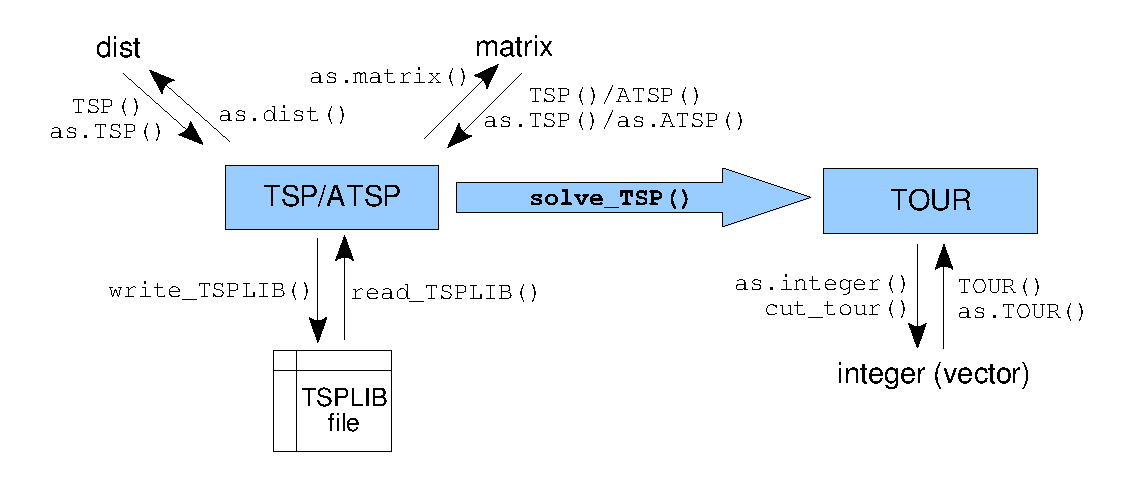
\includegraphics[width=14cm]{overview}
    \caption{An overview of the classes in \pkg{TSP}.\label{fig:overview}}
\end{figure}


\class{TSP} objects can be created from a distance matrix (a
\class{dist} object) or a symmetric matrix using the creator function
\func{TSP} or coercion with \func{as.TSP}.  Similarly, \class{ATSP}
objects are created by \func{ATSP} or \func{as.ATSP} from square
matrices representing the distances.  In the creation process, labels
are taken and stored as city names in the object or can be explicitly
given as arguments to the creator functions.  Several methods are
defined for the classes:
\begin{itemize}
 \item \func{print} displays basic information about the problem (number
  of cities and the distance measure employed).
 \item \func{n\_of\_cities} returns the number of cities.
 \item \func{labels} returns the city names.
 \item \func{image} produces a shaded matrix plot of the distances
  between cities. The order of the cities can be specified as the
  argument \code{order}.
\end{itemize}

Internally, an object of class \class{TSP} is a \class{dist} object with
an additional class attribute and, therefore, if needed, can be coerced
to \class{dist} or to a matrix.  An \class{ATSP} object is represented
as a square matrix.  Obviously, asymmetric TSPs are more general than
symmetric TSPs, hence, symmetric TSPs can also be represented as
asymmetric TSPs.  To formulate an asymmetric TSP as a symmetric TSP with
double the number of cities (see Section \ref{sec:manipulations}),
\func{reformulate\_ATSP\_as\_TSP} is provided.  This function creates
the necessary dummy cities and adapts the distance matrix accordingly.

A popular format to save TSP descriptions to disk which is supported by
most TSP solvers is the format used by \emph{TSPLIB}, a library of
sample instances of the TSP maintained by \cite{Reinelt2004}. The
\pkg{TSP} package provides \func{read\_TSPLIB} and \func{write\_TSPLIB}
to read and save symmetric and asymmetric TSPs in TSPLIB format.

Class \class{TOUR} represents a solution to a TSP by an integer
permutation vector containing the ordered indices and labels of the
cities to visit.  In addition, it stores an attribute indicating the
length of the tour.  Again, suitable \func{print} and \func{labels}
methods are provided.  The raw permutation vector (i.e., the order in
which cities are visited) can be obtained from a tour using
\func{as.integer}.  With \func{cut\_tour}, a circular tour can be split
at a specified city resulting in a path represented by a vector of city
indices.

The length of a tour can always be calculated using \func{tour\_length}
and specifying a TSP and a tour. Instead of the tour, an integer
permutation vector calculated outside the \pkg{TSP} package can be used
as long as it has the correct length.

All TSP solvers in \pkg{TSP} can be used with the simple common interface:

\begin{quote}
\code{solve\_TSP(x, method, control)}   
\end{quote}
where \code{x} is the TSP to be solved, \code{method} is a character
string indicating the method used to solve the TSP and \code{control}
can contain a list with additional information used by the solver.
The available algorithms are shown in Table~\ref{tab:methods}.    

\begin{table}
    \caption{Available algorithms in \pkg{TSP}.}\label{tab:methods}
    \centering
    \begin{tabular}{llc}
    \hline
    \textbf{Algorithm} & \textbf{Method argument} & \textbf{Applicable to} \\
    \hline
    Nearest neighbor algorithm & \code{"nn"} & TSP/ATSP \\
    Repetitive nearest neighbor algorithm & \code{"repetitive\_nn"} 
            & TSP/ATSP \\
    Nearest insertion & \code{"nearest\_insertion"} & TSP/ATSP  \\
    Farthest insertion & \code{"farthest\_insertion"} & TSP/ATSP  \\
    Cheapest insertion & \code{"cheapest\_insertion"} & TSP/ATSP  \\
    Arbitrary insertion & \code{"arbitrary\_insertion"} & TSP/ATSP  \\
    Concorde TSP solver & \code{"concorde"} & TSP  \\
    2-Opt improvement heuristic &  \code{"2-opt"}  & TSP/ATSP \\
    Chained Lin-Kernighan &  \code{"linkern"}  & TSP \\
\hline
\end{tabular}
\end{table}

All algorithms except the Concorde TSP solver and the Chained
Lin-Kernighan heuristic (a Lin-Kernighan variation described in
\cite{Applegate2003}) are included in the package and distributed under
the GNU Public License (GPL). For the Concorde TSP solver and the
Chained Lin-Kernighan heuristic only a simple interface (using
\func{write\_TSPLIB}, calling the executable and reading back the
resulting tour) is included in \pkg{TSP}.  The executable itself is part
of the Concorde distribution, has to be installed separately and is
governed by a different license which allows only for academic use.  The
interfaces are included since
Concorde~\citep{Applegate2000,Applegate2006} is currently one of the
best implementations for solving symmetric TSPs based on the
branch-and-cut method discussed in section~\ref{sec:exact}.  In May
2004, Concorde was used to find the optimal solution for the TSP of
visiting all 24,978 cities in Sweden.  The computation was carried out
on a cluster with 96 Xeon 2.8 GHz nodes and took in total almost 100 CPU
years.

\section{Examples}\label{sec:examples}

In this section we provide some examples for the use of
package~\pkg{TSP}.  We start with a simple example of how to use the
interface of the TSP solver to compare different heuristics.  Then we
show how to solve related tasks, using the Hamiltonian shortest path
problem as an example.  Finally, we give an example of clustering using
the \pkg{TSP} package.  An additional application can be found
in package \pkg{seriation}~\citep{TSP:Hahsler+Buchta+Hornik:2006} which uses
the TSP solvers from \pkg{TSP} to order (seriate) objects given a proximity
matrix.

\subsection{Comparing some heuristics}

In the following example, we use several heuristics to find a short path
in the \code{USCA50} data set which contains the distances between the
first 50 cities in the \code{USCA312} data set. The \code{USCA312} data
set contains the distances between 312 cities in the USA and Canada
coded as a symmetric TSP.  The smaller data set is used here, since some
of the heuristic solvers employed are rather slow.

\begin{Schunk}
\begin{Sinput}
> library("TSP")
> data("USCA50")
> USCA50
\end{Sinput}
\begin{Soutput}
object of class ‘TSP’ 
50 cities (distance ‘euclidean’) 
\end{Soutput}
\end{Schunk}


We calculate tours using different heuristics and store the results in
the list \code{tours}. As an example, we show the first tour which
displays the method employed, the number of cities involved and the tour
length.  All tour lengths are compared using the dot chart in
Figure~\ref{fig:dotchart}.  For the chart, we add a point for the
optimal solution which has a tour length of 14497. The optimal solution
can be found using Concorde (\code{method = "concorde"}).  It is omitted
here, since Concorde has to be installed separately.



\begin{Schunk}
\begin{Sinput}
> methods <- c("nearest_insertion", "farthest_insertion", "cheapest_insertion", 
+     "arbitrary_insertion", "nn", "repetitive_nn", "2-opt")
> tours <- sapply(methods, FUN = function(m) solve_TSP(USCA50, 
+     method = m), simplify = FALSE)
> tours[[1]]
\end{Sinput}
\begin{Soutput}
object of class ‘TOUR’ 
result of method ‘nearest_insertion’ for 50 cities
tour length: 17421 
\end{Soutput}
\begin{Sinput}
> dotchart(c(sapply(tours, FUN = attr, "tour_length"), optimal = 14497), 
+     xlab = "tour length", xlim = c(0, 20000))
\end{Sinput}
\end{Schunk}

\begin{figure}
\centering
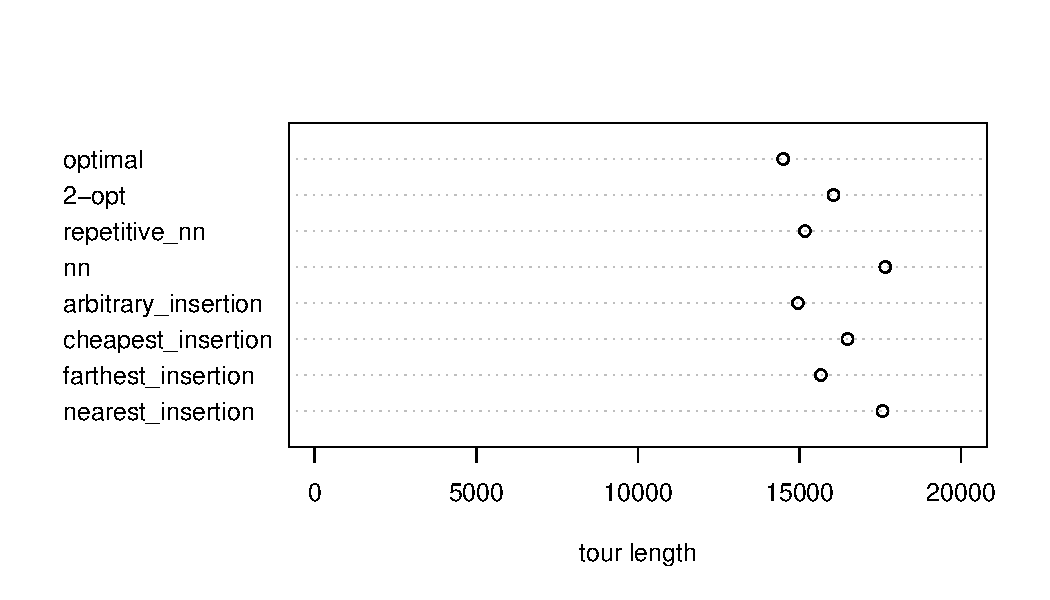
\includegraphics[width=11cm, trim=0 10 0 0]{TSP-dotchart_USCA50}
\caption{Comparison of the tour lengths for the USCA50 data set.}
\label{fig:dotchart}
\end{figure}


\subsection{Finding the shortest Hamiltonian path}

The problem of finding the shortest Hamiltonian path through a graph
(i.e., a path which visits each node in the graph exactly once) can be
transformed into the TSP with cities and distances representing the
graphs vertices and edge weights, respectively~\citep{Garfinkel1985}.

Finding the shortest Hamiltonian path through all cities disregarding
the endpoints can be achieved by inserting a `dummy city' which has a
distance of zero to all other cities. The position of this city in the
final tour represents the cutting point for the path. In the following
we use a heuristic to find a short path in the \code{USCA312} data set.
Inserting dummy cities is performed in \pkg{TSP} by
\func{insert\_dummy}.


\begin{Schunk}
\begin{Sinput}
> library("TSP")
> data("USCA312")
> tsp <- insert_dummy(USCA312, label = "cut")
> tsp
\end{Sinput}
\begin{Soutput}
object of class ‘TSP’ 
313 cities (distance ‘euclidean’) 
\end{Soutput}
\end{Schunk}

The TSP now contains an additional dummy city and we can try to solve
this TSP.

\begin{Schunk}
\begin{Sinput}
> tour <- solve_TSP(tsp, method = "farthest_insertion")
> tour
\end{Sinput}
\begin{Soutput}
object of class ‘TOUR’ 
result of method ‘farthest_insertion’ for 313 cities
tour length: 38184 
\end{Soutput}
\end{Schunk}

Since the dummy city has distance zero to all other cities, the path length is
equal to the tour length reported above. The path starts with the first city in
the list after the `dummy' city  and ends with the city right before it. 
We use \func{cut\_tour} to create a path and show the 
first and last 6 cities on it.

\begin{Schunk}
\begin{Sinput}
> path <- cut_tour(tour, "cut")
> head(labels(path))
\end{Sinput}
\begin{Soutput}
[1] "Lihue, HI"         "Honolulu, HI"      "Hilo, HI"         
[4] "San Francisco, CA" "Berkeley, CA"      "Oakland, CA"      
\end{Soutput}
\begin{Sinput}
> tail(labels(path))
\end{Sinput}
\begin{Soutput}
[1] "Anchorage, AK"     "Fairbanks, AK"     "Dawson, YT"       
[4] "Whitehorse, YK"    "Juneau, AK"        "Prince Rupert, BC"
\end{Soutput}
\end{Schunk}

The tour found in the example results in a path from Lihue on Hawaii to
Prince Rupert in British Columbia. Such a tour can also be visualized
using the packages \pkg{sp}, \pkg{maps} and \pkg{maptools}
\citep{TSP:Pebesma+Bivand:2005}.

\begin{Schunk}
\begin{Sinput}
> library("maps")
> library("sp")
> library("maptools")
> data("USCA312_map")
> plot_path <- function(path) {
+     plot(as(USCA312_coords, "Spatial"), axes = TRUE)
+     plot(USCA312_basemap, add = TRUE, col = "gray")
+     points(USCA312_coords, pch = 3, cex = 0.4, col = "red")
+     path_line <- SpatialLines(list(Lines(list(Line(USCA312_coords[path, 
+         ])))))
+     plot(path_line, add = TRUE, col = "black")
+     points(USCA312_coords[c(head(path, 1), tail(path, 1)), 
+         ], pch = 19, col = "black")
+ }
> plot_path(path)
\end{Sinput}
\end{Schunk}

\begin{figure}
\centering
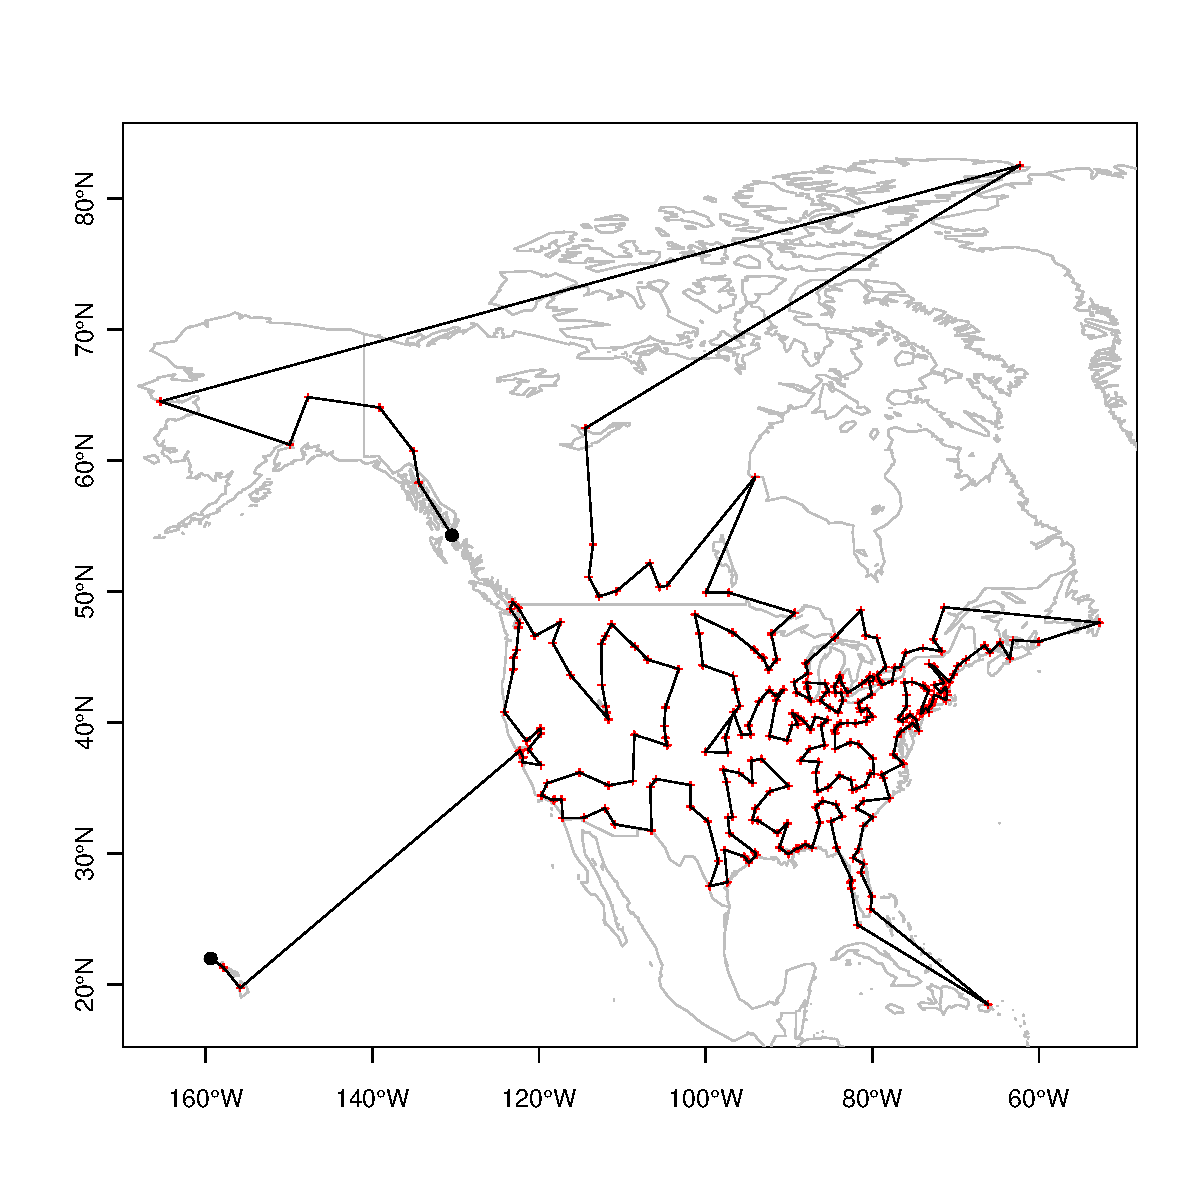
\includegraphics[width=10cm, trim=0 30 0 0]{TSP-map1}
\caption{A ``short'' Hamiltonian path for the USCA312 dataset.}
\label{fig:map1}
\end{figure}

The map containing the path is presented in Figure~\ref{fig:map1}.  It
has to be mentioned that the path found by the used heuristic is
considerable longer than the optimal path found by Concorde with a
length of $34928$, illustrating the power of modern TSP algorithms.

For the following two examples, we indicate how the distance matrix
between cities can be modified to solve related shortest Hamiltonian
path problems.  These examples serve as illustrations of how
modifications can be made to transform different problems into a TSP.

The first problem is to find the shortest Hamiltonian path starting with
a given city. In this case, all distances to the selected city are set
to zero, forcing the evaluation of all possible paths starting with this
city and disregarding the way back from the final city in the tour.  By
modifying the distances the symmetric TSP is changed into an asymmetric
TSP (ATSP) since the distances between the starting city and all other
cities are no longer symmetric.

As an example, we choose New York as the starting city.  We transform
the data set into an ATSP and set the column corresponding to New York
to zero before solving it.  Thus, the distance to return from the last
city in the path to New York does not contribute to the path length.  We
use the nearest neighbor heuristic to calculate an initial tour which is
then improved using $2$-Opt moves and cut at New York to create a path.



\begin{Schunk}
\begin{Sinput}
> atsp <- as.ATSP(USCA312)
> ny <- which(labels(USCA312) == "New York, NY")
> atsp[, ny] <- 0
> initial_tour <- solve_TSP(atsp, method = "nn")
> initial_tour
\end{Sinput}
\begin{Soutput}
object of class ‘TOUR’ 
result of method ‘nn’ for 312 cities
tour length: 49697 
\end{Soutput}
\begin{Sinput}
> tour <- solve_TSP(atsp, method = "2-opt", control = list(tour = initial_tour))
> tour
\end{Sinput}
\begin{Soutput}
object of class ‘TOUR’ 
result of method ‘2-opt’ for 312 cities
tour length: 39445 
\end{Soutput}
\begin{Sinput}
> path <- cut_tour(tour, ny, exclude_cut = FALSE)
> head(labels(path))
\end{Sinput}
\begin{Soutput}
[1] "New York, NY"    "Jersey City, NJ" "Elizabeth, NJ"   "Newark, NJ"     
[5] "Paterson, NJ"    "Binghamtom, NY" 
\end{Soutput}
\begin{Sinput}
> tail(labels(path))
\end{Sinput}
\begin{Soutput}
[1] "Edmonton, AB"  "Saskatoon, SK" "Moose Jaw, SK" "Regina, SK"   
[5] "Minot, ND"     "Brandon, MB"  
\end{Soutput}
\end{Schunk}
\begin{Schunk}
\begin{Sinput}
> plot_path(path)
\end{Sinput}
\end{Schunk}

\begin{figure}
\centering
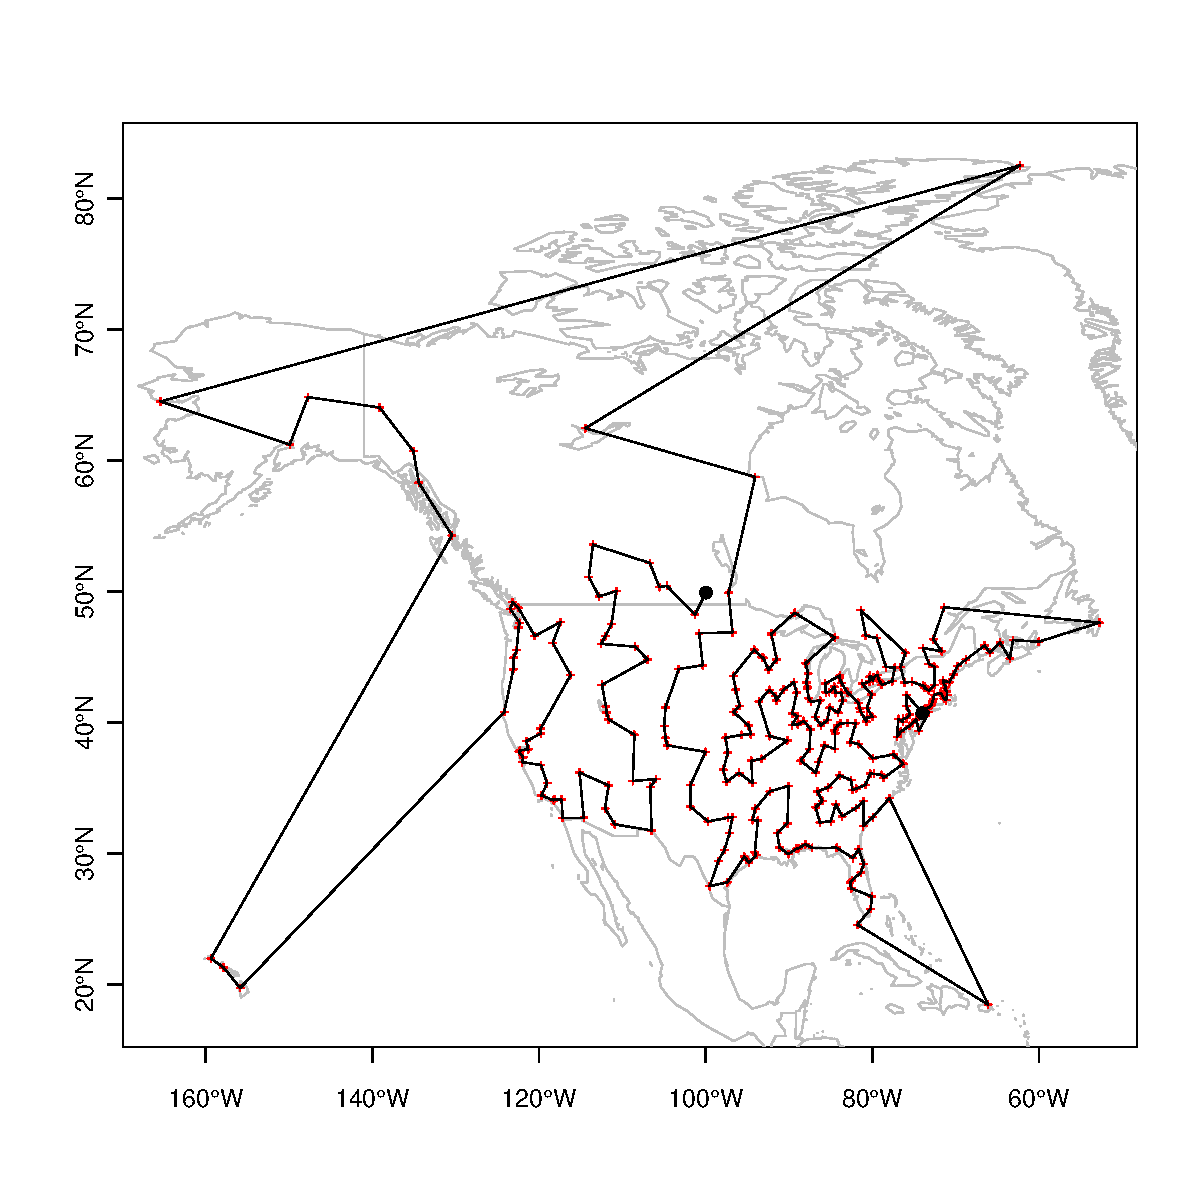
\includegraphics[width=10cm, trim=0 30 0 0]{TSP-map2}
\caption{A Hamiltonian path for the USCA312 dataset starting in New York.}
\label{fig:map2}
\end{figure}

The found path is presented in Figure~\ref{fig:map2}. It begins with New
York and cities in New Jersey and ends in a city in Manitoba, Canada.
%The path shows the typical behavior 
%of the nearest neighbor heuristic with first connecting the cities close by and
%then making rather big ``jumps'' for the final cities.

Concorde and many advanced TSP solvers can only solve symmetric TSPs. To
use these solvers, we can formulate the ATSP as a TSP using
\func{reformulate\_ATSP\_as\_TSP} which introduces a dummy city for each
city (see Section~\ref{sec:manipulations}).

\begin{Schunk}
\begin{Sinput}
> tsp <- reformulate_ATSP_as_TSP(atsp)
> tsp
\end{Sinput}
\begin{Soutput}
object of class ‘TSP’ 
624 cities (distance ‘unknown’) 
\end{Soutput}
\end{Schunk}

After finding a tour for the TSP, the dummy cities are removed again giving the
tour for the original ATSP.  
Note that the tour needs to be reversed if the
dummy cities appear before and not after the original cities in the solution of
the TSP.  The following code is not executed here, since it takes several
minutes to execute and Concorde has to be installed separately.  Concorde finds
the optimal solution with a length of $36091$.


\begin{Schunk}
\begin{Sinput}
> tour <- solve_TSP(tsp, method = "concorde")
> tour <- as.TOUR(tour[tour <= n_of_cities(atsp)])
\end{Sinput}
\end{Schunk}


Finding the shortest Hamiltonian path which ends in a given city can be
achieved likewise by setting the row in the distance matrix which
corresponds to this city to zero.

For finding the shortest Hamiltonian path we can also restrict both end
points.  This problem can be transformed to a TSP by replacing the two
cities by a single city which contains the distances from the start
point in the columns and the distances to the end point in the
rows. Obviously this is again an asymmetric TSP.

For the following example, we are only interested in paths starting in
New York and ending in Los Angeles. Therefore, we remove the two cities
from the distance matrix, create an asymmetric TSP and insert a dummy
city called \code{"LA/NY"}. The distances from this dummy city are
replaced by the distances from New York and the distances towards are
replaced by the distances towards Los Angeles.



\begin{Schunk}
\begin{Sinput}
> m <- as.matrix(USCA312)
> ny <- which(labels(USCA312) == "New York, NY")
> la <- which(labels(USCA312) == "Los Angeles, CA")
> atsp <- ATSP(m[-c(ny, la), -c(ny, la)])
> atsp <- insert_dummy(atsp, label = "LA/NY")
> la_ny <- which(labels(atsp) == "LA/NY")
> atsp[la_ny, ] <- c(m[-c(ny, la), ny], 0)
> atsp[, la_ny] <- c(m[la, -c(ny, la)], 0)
\end{Sinput}
\end{Schunk}


We use the nearest insertion heuristic.
\begin{Schunk}
\begin{Sinput}
> tour <- solve_TSP(atsp, method = "nearest_insertion")
> tour
\end{Sinput}
\begin{Soutput}
object of class ‘TOUR’ 
result of method ‘nearest_insertion’ for 311 cities
tour length: 45029 
\end{Soutput}
\begin{Sinput}
> path_labels <- c("New York, NY", labels(cut_tour(tour, la_ny)), 
+     "Los Angeles, CA")
> path_ids <- match(path_labels, labels(USCA312))
> head(path_labels)
\end{Sinput}
\begin{Soutput}
[1] "New York, NY"        "North Bay, ON"       "Sudbury, ON"        
[4] "Timmins, ON"         "Sault Ste Marie, ON" "Thunder Bay, ON"    
\end{Soutput}
\begin{Sinput}
> tail(path_labels)
\end{Sinput}
\begin{Soutput}
[1] "Eureka, CA"        "Reno, NV"          "Carson City, NV"  
[4] "Stockton, CA"      "Santa Barbara, CA" "Los Angeles, CA"  
\end{Soutput}
\end{Schunk}
\begin{Schunk}
\begin{Sinput}
> plot_path(path_ids)
\end{Sinput}
\end{Schunk}


The path jumps from New York to cities in Ontario and it passes through
cities in California and Nevada before ending in Los Angeles. The path
displayed in Figure~\ref{fig:map3} contains multiple crossings which
indicate that the solution is suboptimal. The optimal solution generated
by reformulating the problem as a TSP and using Concorde has only a tour
length of $38489$.

\begin{figure}
\centering
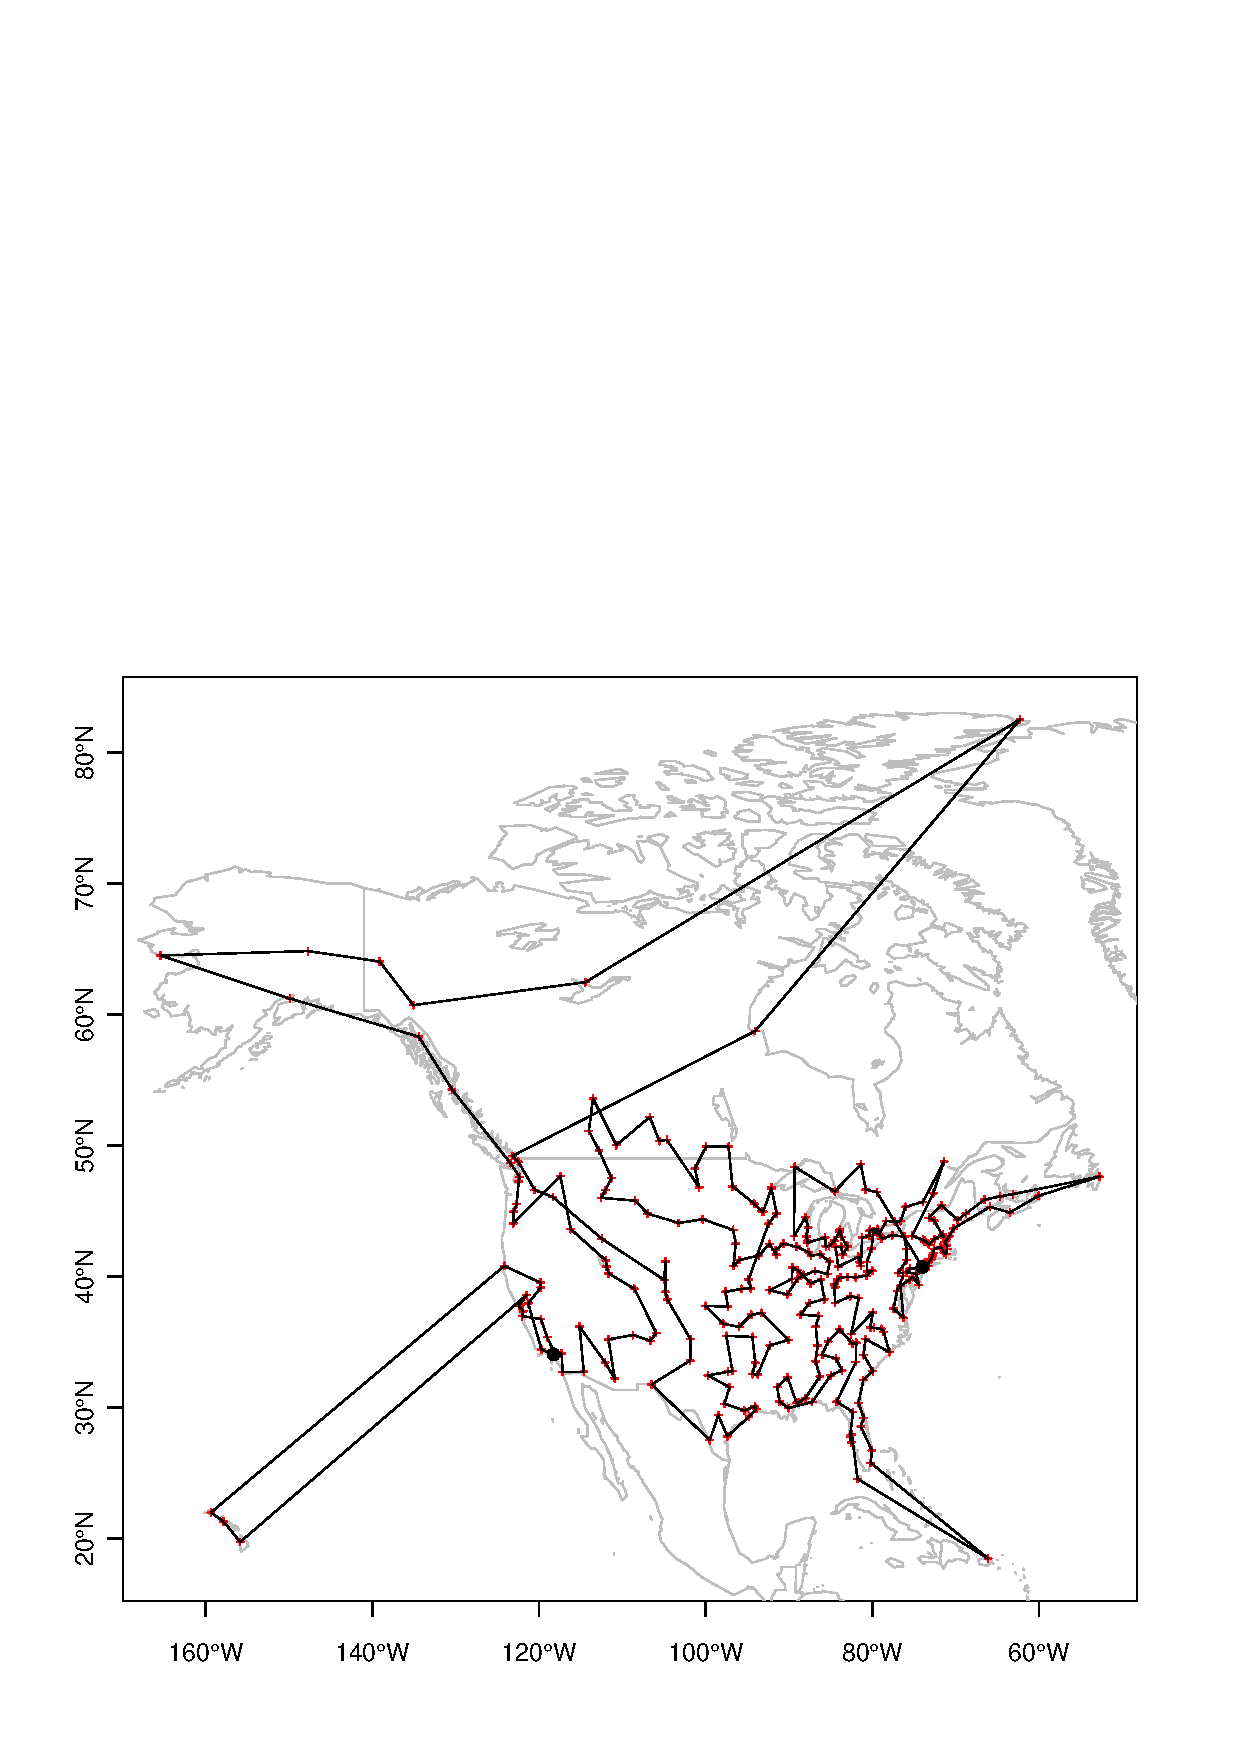
\includegraphics[width=10cm, trim=0 30 0 0]{TSP-map3}
\caption{A Hamiltonian path for the USCA312 dataset starting in New York
  and ending in Los Angles.}
\label{fig:map3}
\end{figure}


\subsection{Rearrangement clustering}
Solving a TSP to obtain a clustering was suggested several times in the
literature \citep[see, e.g.,][]{Lenstra1974, Alpert1997, Johnson2004}.  The idea
is that objects in clusters are visited in consecutive order and from one
cluster to the next larger ``jumps'' are necessary.  \cite{Climer2006} call
this type of clustering \emph{rearrangement clustering} and suggest to
automatically find the cluster boundaries of $k$ clusters by adding $k$
\emph{dummy cities} which have constant distance $c$ to all other cities and
are infinitely far from each other. In the optimal
solution of the TSP, the dummy cities must separate the most distant cities and
thus represent optimal boundaries for $k$ clusters.

For the following example, we use the well known iris data set. Since we
know that the dataset contains three classes denoted by the variable
\code{Species}, we insert three dummy cities into the TSP for the iris
data set and perform rearrangement clustering using the default method
(nearest insertion algorithm).  Note that this algorithm does not find
the optimal solution and it is not guaranteed that the dummy cities will
present the best cluster boundaries.
%\marginpar{FIXME: Was sagt Concorde dazu?}

\begin{Schunk}
\begin{Sinput}
> data("iris")
> tsp <- TSP(dist(iris[-5]), labels = iris[, "Species"])
> tsp_dummy <- insert_dummy(tsp, n = 3, label = "boundary")
> tour <- solve_TSP(tsp_dummy)
\end{Sinput}
\end{Schunk}

Next, we plot the TSP's permuted distance matrix using shading to
represent distances. The result is displayed as
Figure~\ref{fig:clustering}. Lighter areas represent larger
distances. The additional red lines represent the positions of the dummy
cities in the tour, which mark the cluster boundaries obtained.


\begin{Schunk}
\begin{Sinput}
> image(tsp_dummy, tour, xlab = "objects", ylab = "objects")
> abline(h = which(labels(tour) == "boundary"), col = "red")
> abline(v = which(labels(tour) == "boundary"), col = "red")
\end{Sinput}
\end{Schunk}


\begin{figure}
\centering
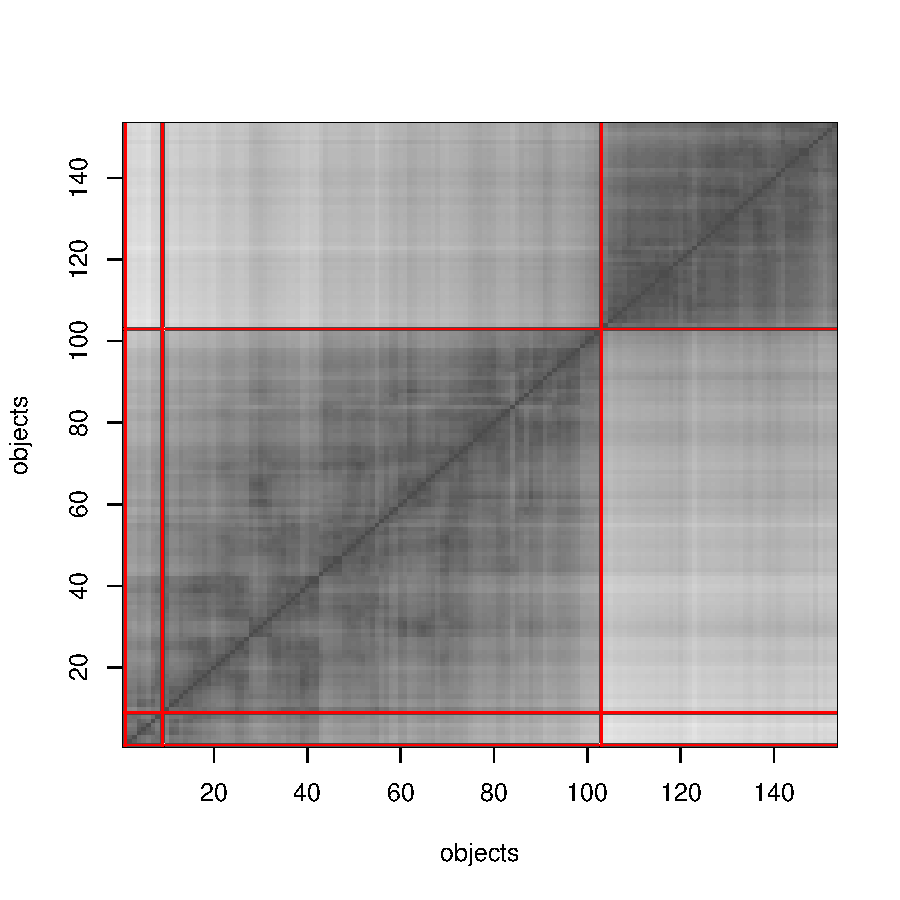
\includegraphics[width=9cm, height=9cm, trim=0 20 0 0]{TSP-clustering}
\caption{Result of rearrangement clustering using three dummy cities and the 
nearest insertion algorithm on the iris data set.}
\label{fig:clustering}
\end{figure}


One pair of red horizontal and vertical lines exactly separates the
darker from lighter areas.  The second pair occurs inside the larger
dark block.  We can look at how well the partitioning obtained fits the
structure in the data given by the species field in the data set.  Since
we used the species as the city labels in the TSP, the labels in the
tour represent the partitioning with the dummy cities named `boundary'
separating groups.  The result can be summarized based on the run length
encoding of the obtained tour labels:

\begin{Schunk}
\begin{Sinput}
> out <- rle(labels(tour))
> data.frame(Species = out$values, Lenghts = out$lengths, Pos = cumsum(out$lengths))
\end{Sinput}
\begin{Soutput}
      Species Lenghts Pos
1    boundary       1   1
2   virginica       7   8
3    boundary       1   9
4   virginica      18  27
5  versicolor       5  32
6   virginica      20  52
7  versicolor       1  53
8   virginica       3  56
9  versicolor      13  69
10  virginica       1  70
11 versicolor      13  83
12  virginica       1  84
13 versicolor      18 102
14   boundary       1 103
15     setosa      50 153
\end{Soutput}
\end{Schunk}


One boundary perfectly splits the iris data set into a group containing
only examples of species `Setosa' and a second group containing examples
for `Virginica' and `Versicolor'.  However, the second boundary only
separates several examples of species `Virginica' from other examples of
the same species.  Even in the optimal tour found by Concorde, this
problem occurs. The reason why the rearrangement clustering fails to
split the data into three groups is the closeness between the groups
`Virginica' and `Versicolor'.  To inspect this problem further, we can
project the data points on the first two principal components of the
data set and add the path segments which resulted from solving the TSP.

\begin{Schunk}
\begin{Sinput}
> prc <- prcomp(iris[1:4])
> plot(prc$x, pch = as.numeric(iris[, 5]), col = as.numeric(iris[, 
+     5]))
> indices <- c(tour, tour[1])
> indices[indices > 150] <- NA
> lines(prc$x[indices, ])
\end{Sinput}
\end{Schunk}

\begin{figure}
\centering
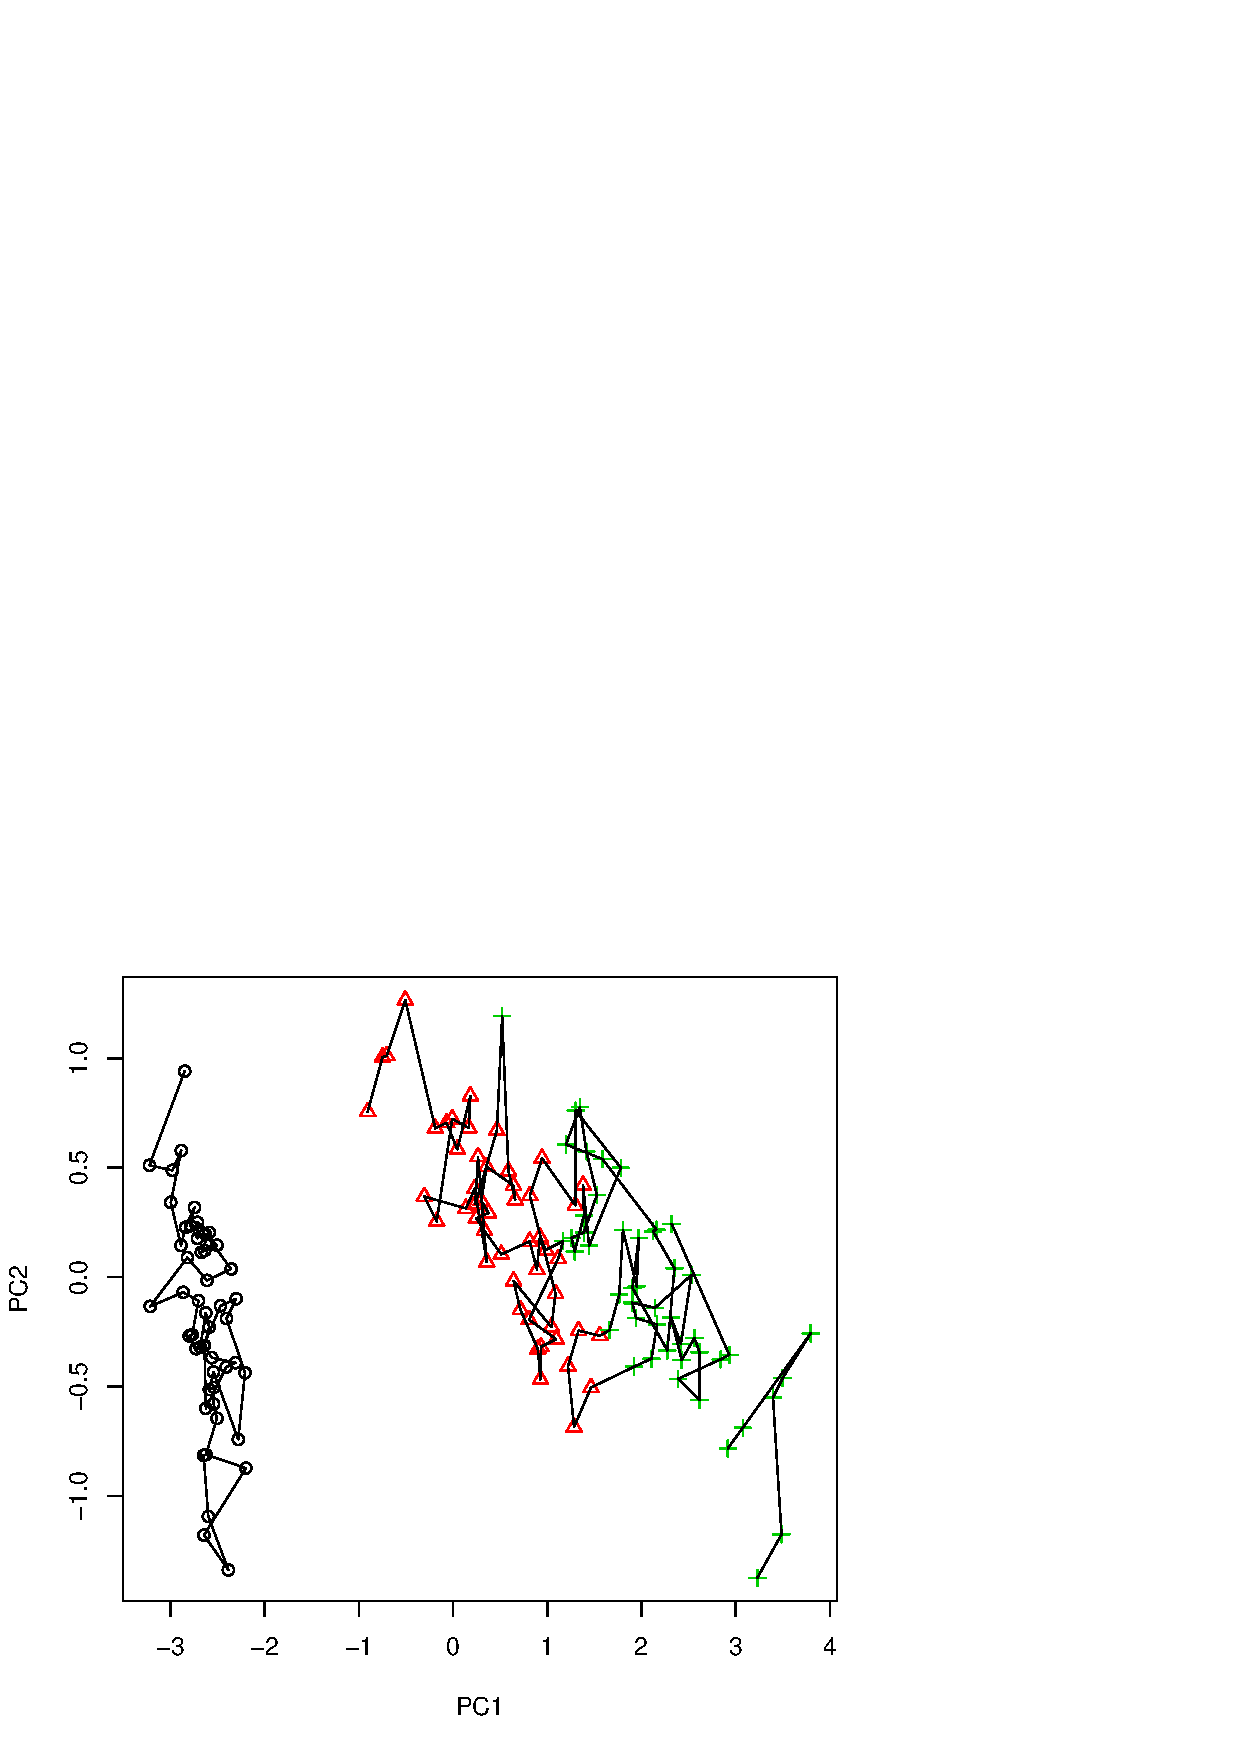
\includegraphics[width=10cm, trim=0 20 0 0]{TSP-clustering2}
\caption{The 3 path segments representing a rearrangement clustering of the
iris data set.  The data points are projected on the set's first two principal
components.  The three species are represented by different markers and
colors.}
\label{fig:clustering2}
\end{figure}

The result in shown in Figure~\ref{fig:clustering2}.  The three species
are identified by different markers and all points connected by a single
path represent a cluster found.  Clearly, the two groups to the right
side of the plot are too close to be separated correctly by using just
the distances between individual points.  This problem is similar to the
\emph{chaining effect} known from hierarchical clustering using the
single-linkage method.

\section{Conclusion}\label{sec:conclusion}

In this paper we presented the R extension package \pkg{TSP} which
implements an infrastructure to handle and solve TSPs. The package
introduces classes for problem descriptions (\class{TSP} and
\class{ATSP}) and for the solution (\class{TOUR}).  Together with a
simple interface for solving TSPs, it allows for an easy and transparent
usage of the package.

With the interface to Concorde, \pkg{TSP} also can use a state of the
art implementation which efficiently computes exact solutions using
branch-and-cut.

\section*{Acknowledgments}

The authors of this paper want to thank Roger Bivand for providing the
code to correctly draw tours and paths on a projected map.


%
\bibliographystyle{abbrvnat}
\bibliography{TSP}
%
\end{document}

